% Made up for the tikra benchmark.
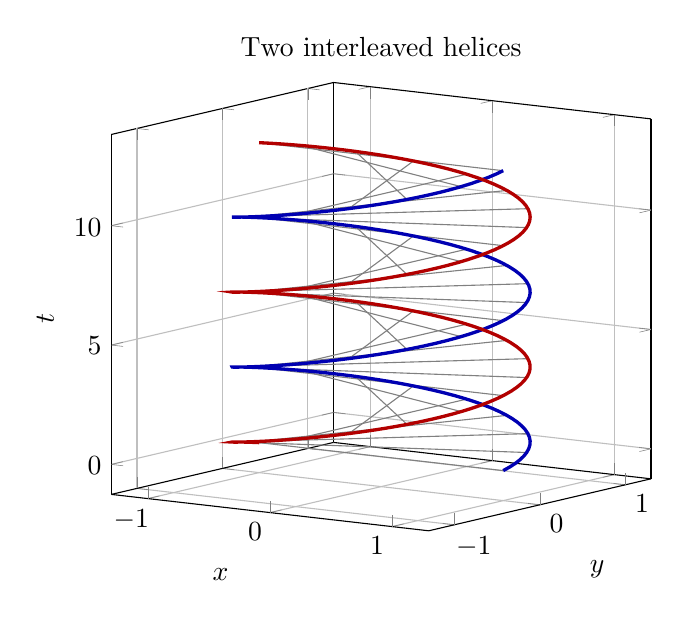
\begin{tikzpicture}
\begin{axis}[view={35}{10}, xlabel=$x$, ylabel=$y$, zlabel=$t$,
    title={Two interleaved helices}, grid=major, xmin=-1.3, xmax=1.3, ymin=-1.3, ymax=1.3]
  \addplot3[gray, thin, samples=33, domain=0:4*pi, samples y=0, variable=\t,
      quiver={u=-2*x, v=-2*y, w=0}, -]
    ({cos(deg(t))}, {sin(deg(t))}, {t});
  \addplot3[very thick, blue!70!black, samples=160, domain=0:4*pi, samples y=0]
    ({cos(deg(x))}, {sin(deg(x))}, {x});
  \addplot3[very thick, red!70!black, samples=160, domain=0:4*pi, samples y=0]
    ({-cos(deg(x))}, {-sin(deg(x))}, {x});
\end{axis}
\end{tikzpicture}
